\documentclass[a4paper,openright,twoside]{memoir}
\usepackage[utf8]{inputenc}
\usepackage[english]{babel}
\usepackage{geometry}
\usepackage{graphicx}
\usepackage{amsmath}
\usepackage{microtype}
\usepackage{nicefrac}
\usepackage{bm}
\usepackage{geometry}
\usepackage{natbib}
\usepackage{booktabs}

\setsecnumdepth{subsection}
\settocdepth{section}
\chapterstyle{section}
\nouppercaseheads
\setlength{\parskip}{0.1 cm}

\begin{document}

% boring frontpage
\begin{titlingpage}
\centering
\vspace*{1cm}
\hrule
\vspace*{1cm}
{\huge \textsf{\LaTeX \, Course}}

\vspace*{8mm}
\hrule
\vspace*{1cm}
\textbf{by Tim Birger Tejsner}

\vfill

\small Supervisor: Noone

\vspace*{1cm}

\textsc{Independent Project\\ \today}

\textsc{\textsc{Roskilde University}}
\end{titlingpage}

\tableofcontents*

\chapter{Introduction}
Lorem ipsum dolor sit amet, consectetur adipiscing elit. Etiam vel neque eu neque molestie gravida. Curabitur in sodales enim. Sed vitae nulla dignissim, dapibus sem accumsan, blandit risus. Cras ac nisi dapibus, ornare justo et, placerat urna. Aenean rutrum tempor ex at accumsan. Maecenas varius, tortor quis facilisis mollis, justo mi consequat massa, at tristique lorem quam ac justo. Cras ut fermentum ligula, vel rutrum mi.

Vestibulum id tellus in nunc ornare consectetur eget et purus. Donec vitae dui et sem blandit dignissim. Praesent semper nisl ac nunc faucibus fermentum. Proin eu faucibus lacus, id ornare nibh. Quisque in ante justo. Integer quis nisl tempus, fringilla neque a, tempor turpis. Nulla vitae nulla vitae ligula rutrum accumsan. Mauris nec ornare justo. Morbi luctus ullamcorper felis, maximus pharetra leo gravida quis.

In congue in lectus in laoreet. Donec sed dui ipsum. Maecenas at maximus enim, eu auctor tellus. Phasellus maximus velit at dolor convallis molestie. Aliquam viverra efficitur maximus. Proin condimentum, libero at malesuada lobortis, risus lectus scelerisque leo, et egestas turpis urna at ex. Suspendisse ut est eu orci viverra sagittis non vel dui. Vivamus et massa molestie, consequat erat nec, suscipit sem. Maecenas pulvinar velit quis enim hendrerit dapibus. Nunc ut mauris id diam posuere tristique. Fusce convallis tellus quis dui dapibus hendrerit. Cras malesuada finibus erat sit amet maximus.

Vivamus quis nibh dapibus, sagittis dolor a, viverra metus. Etiam in commodo erat, vitae fermentum lectus. Ut finibus, nisl vel ornare lacinia, ipsum ex dapibus nunc, quis ultricies sem nulla quis metus. Nullam metus diam, convallis faucibus urna a, suscipit molestie libero. In eget ligula laoreet, malesuada metus at, pretium metus. Morbi faucibus, nibh id fermentum mollis, sapien nunc bibendum augue, ac semper nunc augue vel nibh. Integer mollis porttitor eros, et tristique turpis mollis quis. Proin cursus vel leo vitae porta. Vestibulum condimentum ex ut sapien tempus, at interdum mauris blandit. Duis in vehicula nisl, sit amet commodo eros. Morbi a varius augue. Proin ultricies sem et neque euismod, at feugiat lectus scelerisque.


\section{Section}
Lorem ipsum dolor sit amet, consectetur adipiscing elit. Mauris id ultricies nulla, et blandit mi. Duis eu nisl vel dolor ultrices sollicitudin eget vitae augue. Fusce varius dignissim dolor, eget congue enim porttitor sit amet. Integer urna eros, rutrum et metus ac, luctus gravida purus. Praesent porttitor placerat hendrerit. Proin vestibulum dignissim sem, in tempor sapien consequat ac. Sed tincidunt ipsum vel sapien pulvinar, quis tempus urna efficitur. Aliquam aliquet orci et fringilla pellentesque. Suspendisse et malesuada eros. Phasellus eros erat, iaculis et mollis vel, tempus nec lacus.

Praesent volutpat imperdiet ante nec placerat. Pellentesque interdum tellus in auctor maximus. Sed posuere faucibus ligula, ac tempus felis cursus dictum. Nulla consectetur tincidunt quam non tincidunt. Aenean magna dui, rhoncus non finibus ut, faucibus vel lacus. Cras in commodo lacus. Ut sed orci eu dolor egestas viverra. Mauris pretium libero ut tellus congue pharetra. Vestibulum sodales enim vel tortor tristique, quis tempus ipsum varius. Quisque congue leo vel sodales maximus. Sed eu tincidunt leo, in laoreet magna. Curabitur faucibus, urna sed placerat porttitor, lorem mauris pharetra lacus, vitae elementum enim nunc consectetur lectus. Etiam cursus erat lorem, posuere vehicula arcu eleifend nec. Nam egestas leo vitae odio mattis congue.

Cras mollis velit quis pulvinar efficitur. Vestibulum facilisis cursus maximus. Integer vitae aliquet ligula, vel lobortis dui. Vestibulum libero libero, luctus in mi vitae, pretium molestie erat. Donec condimentum gravida erat, ut venenatis enim. Duis at metus commodo, pulvinar sem sed, aliquam nunc. Sed rhoncus nulla luctus neque venenatis malesuada eget a mauris. Donec felis tellus, mollis a tempus quis, porta in leo. Lorem ipsum dolor sit amet, consectetur adipiscing elit. Mauris tincidunt finibus neque nec hendrerit. Aliquam dictum turpis eleifend pretium tincidunt.

\begin{itemize}
\item Lorem
\item Dolor 
\item Amet
\end{itemize}


\chapter{Theory}

Here lies some math heavy stuff

\[ E = mc^2 \]

\chapter{Analysis}

In Figure \ref{fig:xray} we see an an illustration of a scattering experiment, and Table \ref{tab:planet-data} contains some planet data!

\begin{figure}
\centering
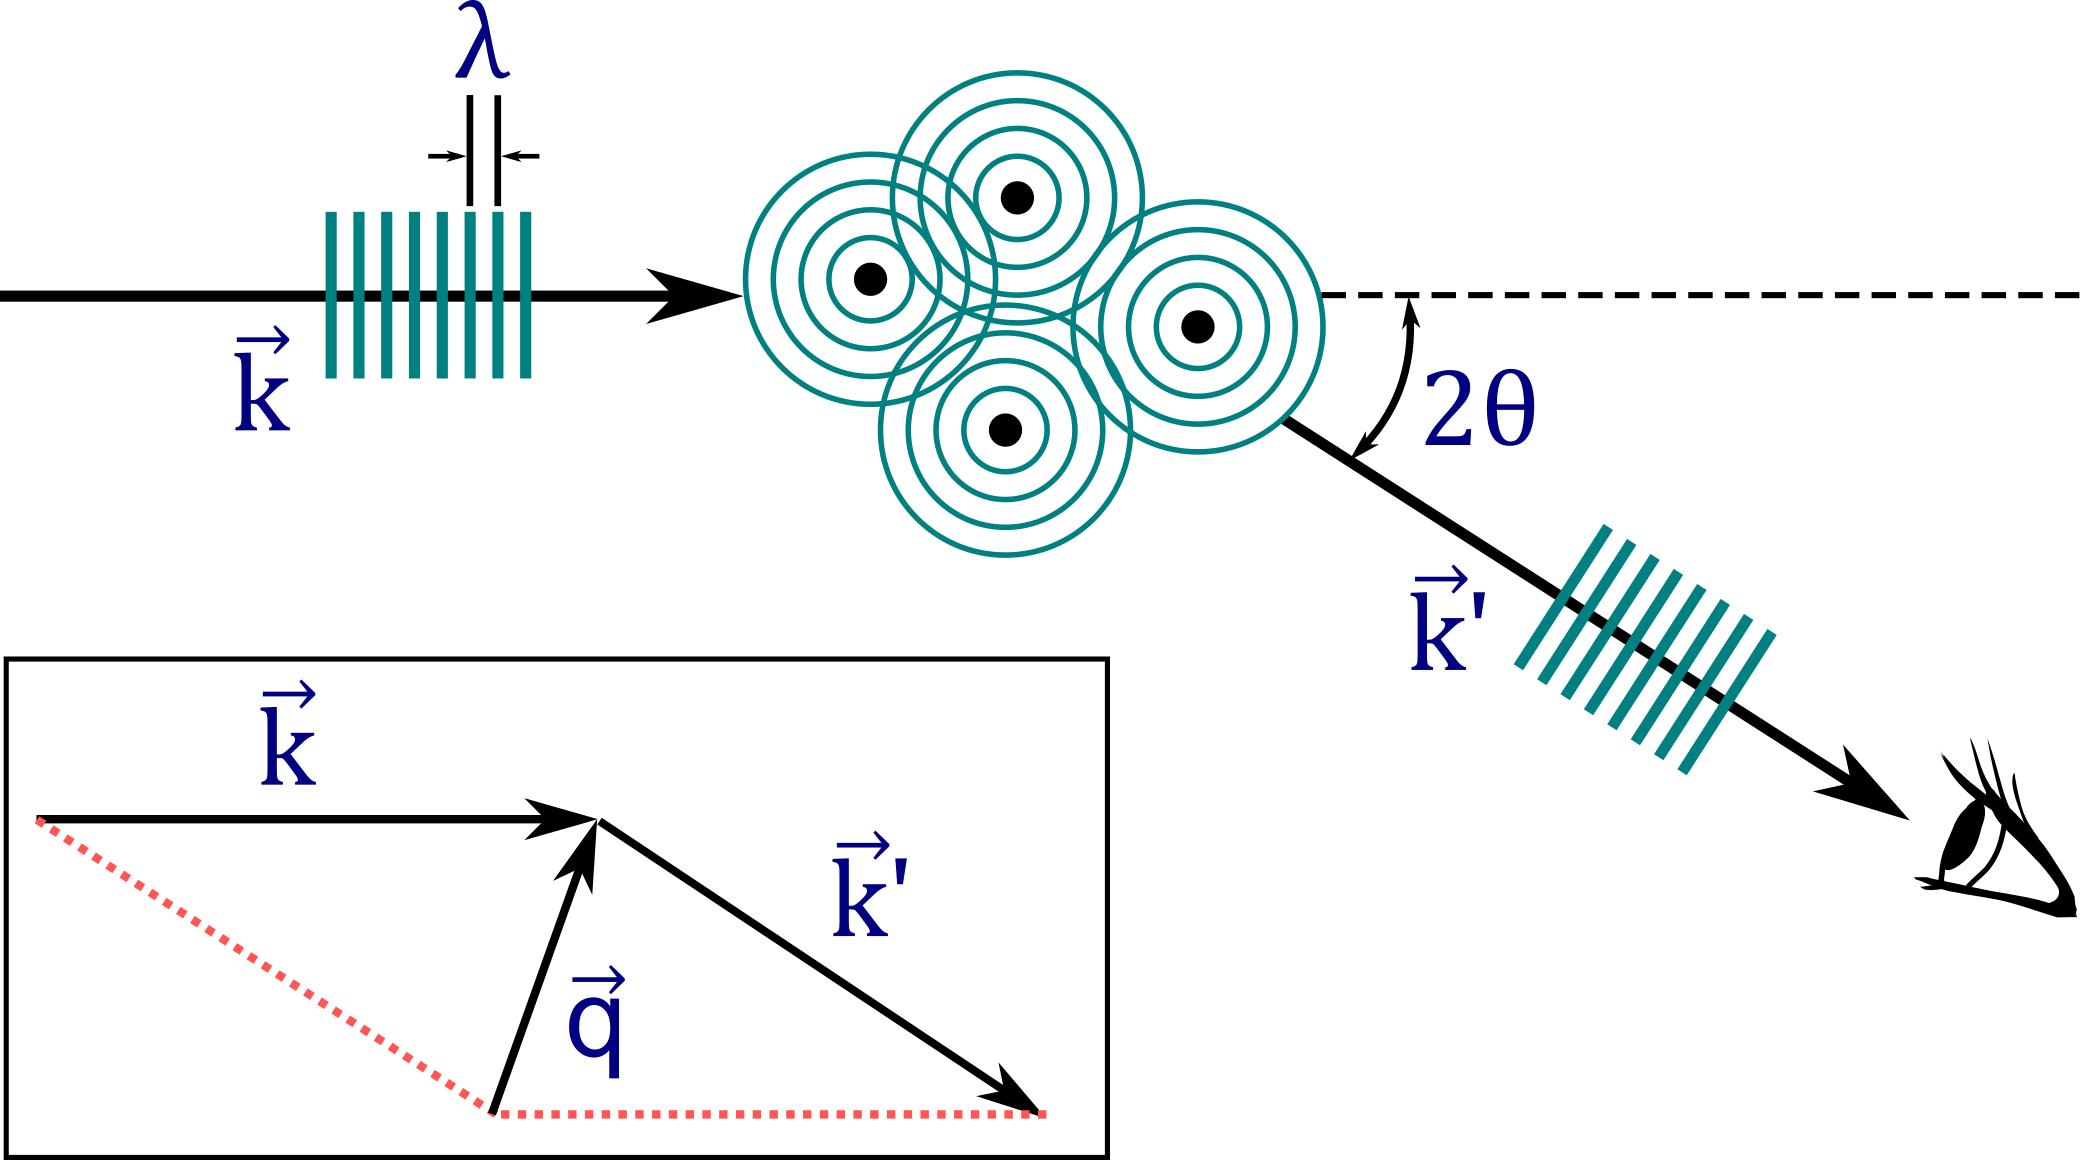
\includegraphics[width=0.6\textwidth]{img/xray.png}
\caption{The archetypical X-ray scattering experiment.}
\label{fig:xray}
\end{figure}

\begin{table}
\centering
\caption{Mass and radii of planets in our solar system.}
\label{tab:planet-data}
\begin{tabular}{@{}lll@{}}
\toprule
Planet & Radius (km) & Mass (kg) \\
\midrule
Mercury & 2440 & $3.30 \cdot 10^{23}$ \\
Venus & 6052 & $4.87 \cdot 10^{24}$ \\
Earth & 6378 & $5.97 \cdot 10^{24}$ \\
Mars & 3397 & $6.42\cdot 10^{23}$ \\
Jupiter & 71492 & $1.90\cdot 10^{27}$ \\
Saturn & 60268 & $5.68 \cdot 10^{26}$ \\
Uranus & 25559 & $8.68 \cdot 10^{25}$ \\
Neptune & 24766 & $1.02 \cdot 10^{26}$ \\ 
\bottomrule
\end{tabular}
\end{table}

\nocite{*}
\bibliographystyle{unsrt}
\bibliography{bibliography}

\end{document}


% wizard til tabeller i texmaker
% matematik: align, integraler, differentiere, sumtegn
% hvordan babel virker
% opsætning af litteraturliste
% forside miniprojekt
% website litteraturliste
% excel konverter

